% $Id: conclusion.tex 
% !TEX root = main.tex

%%
\section{Validation}
\label{sec:validation}

%%%%
\subsection{Evaluation scenarios}
To evaluate the effectiveness of \adaptiverl in adapting to changing goals and new acquired actions we tuse two different scenarios. First, we use the Gridworld benchmark as a proof of concept evaluation and running example of \adaptiverl. Second we use a traffic-signal control scenario to validate adaptation under real-world scenarios.

%%%%%%
\subsubsection{Gridworld}
After every 300 episodes --by 
which time the agent should have learned the optimal policy---we trigger a concept drift by relocating 
the goal to the diagonally opposite corner (bottom-right). We repeat this alternation for a total of $1,500$ 
episodes, expecting the agent to detect each drift and re-converge to the new optimal policy

%%%%%%
\subsubsection{Traffic-signal control}
Intelligent traffic management is a canonical application of self-adaptive systems~\cite{HENRICHS2022106940}, and recent meta-\ac{RL} work has shown benefits when reward functions change with traffic saturation~\cite{meta-rl-traffic}. Here, we model two crossing lanes (C1 vertical, C2 horizontal) with Poisson arrivals and dynamically switch congestion levels (changing $\lambda$ parameter) to induce concept drift. 

We implement a custom \texttt{TrafficEnv} (extending OpenAI's Gym library~\cite{gymlib}) whose state is $(c_1,c_2)$, the number of queued vehicles on lanes C1 and C2 (each in $[0,\mathit{max\_state}]$). At each time step the agent selects one of three signal phases (actions): $\{\,(5,2),\;(2,5),\;(3,3)\}$, indicating service capacities (percentage of the lane cleared per step) for C1 and C2, respectively. During each step, service is applied to C1, new vehicles arrive to C2 (Poisson with rate $\lambda_{2}$), then service is applied to C2, followed by arrivals to C1 (Poisson with rate $\lambda_{1}$). Any unused service capacity incurs a penalty:
\[
\mathrm{penalty} \;=\; 3\times(\text{waste}_{C1} + \text{waste}_{C2})\,,
\]
discouraging “over-serving” when queues are small.

The \emph{dynamic reward} combines congestion cost and service penalty:
\[
r = 
\begin{cases}
-(2c_1 + c_2)\quad &\text{if }c_1>7 \;\wedge\;c_1>c_2,\\
-(c_1 + 2c_2)\quad &\text{if }c_2>7 \;\wedge\;c_2>c_1,\\
-(c_1 + c_2)\quad &\text{otherwise}
\end{cases}
\;-\;\mathrm{penalty}\,
\]
Episodes last 30 steps. We induce two concept drifts by changing arrival rates at episodes 3,000 and 8,000 for a total run of 10,000 episodes:
\[
(\lambda_1,\lambda_2):
\;(4,2)\;\to\;(5,7)\;\to\;(3,1)
\]

Note that when a drift is detected, agents \emph{append} two new phases:
$(7,3)$ and $(3,7)$, allowing for finer control under high congestion. Old actions are never removed.

%%%
\subsection{Experimental setting}
All experiments are run on an Intel Core i5 with 64GB RAM. The experiments use version 3.12 of Python with the Gym library (0.26.2). 

For the evaluation in both application domains we compare the standard Q-learning algorithm (used as a baseline) and \adaptiverl.
\begin{itemize}
  \item \emph{standard Q-learning} agents are defined with a fixed $\alpha=0.1$, and $\varepsilon$ decayed exponentially to $0.01$ from $0.9$.
  \item \adaptiverl agents use the PH-test to detect drifts in episode-rewards, resets $\varepsilon\!=\!1$ upon detection, and adaptively adjusts $\alpha$ based on the TD-error (\cf. \fref{sec:implementation}).  
\end{itemize}

%%%%
\subsection{Evaluation results}

%%%%%%
\subsubsection{Gridworld}


%%%%%%
\subsubsection{Traffic-signal control}

We now focus on the results of using \adaptiverl in a realistic traffic-signal control scenario under non-stationary congestion.  

\fref{fig:traffic-learning-curve} plots the cumulative mean reward (over the last 500 episodes) for both agents. The green vertical line marks the PH-test detection at episode 3004; the second drift at episode 8000 was not flagged, since the new arrival rates produce a reward distribution within the original sensitivity threshold.

\begin{figure*}
    \centering
    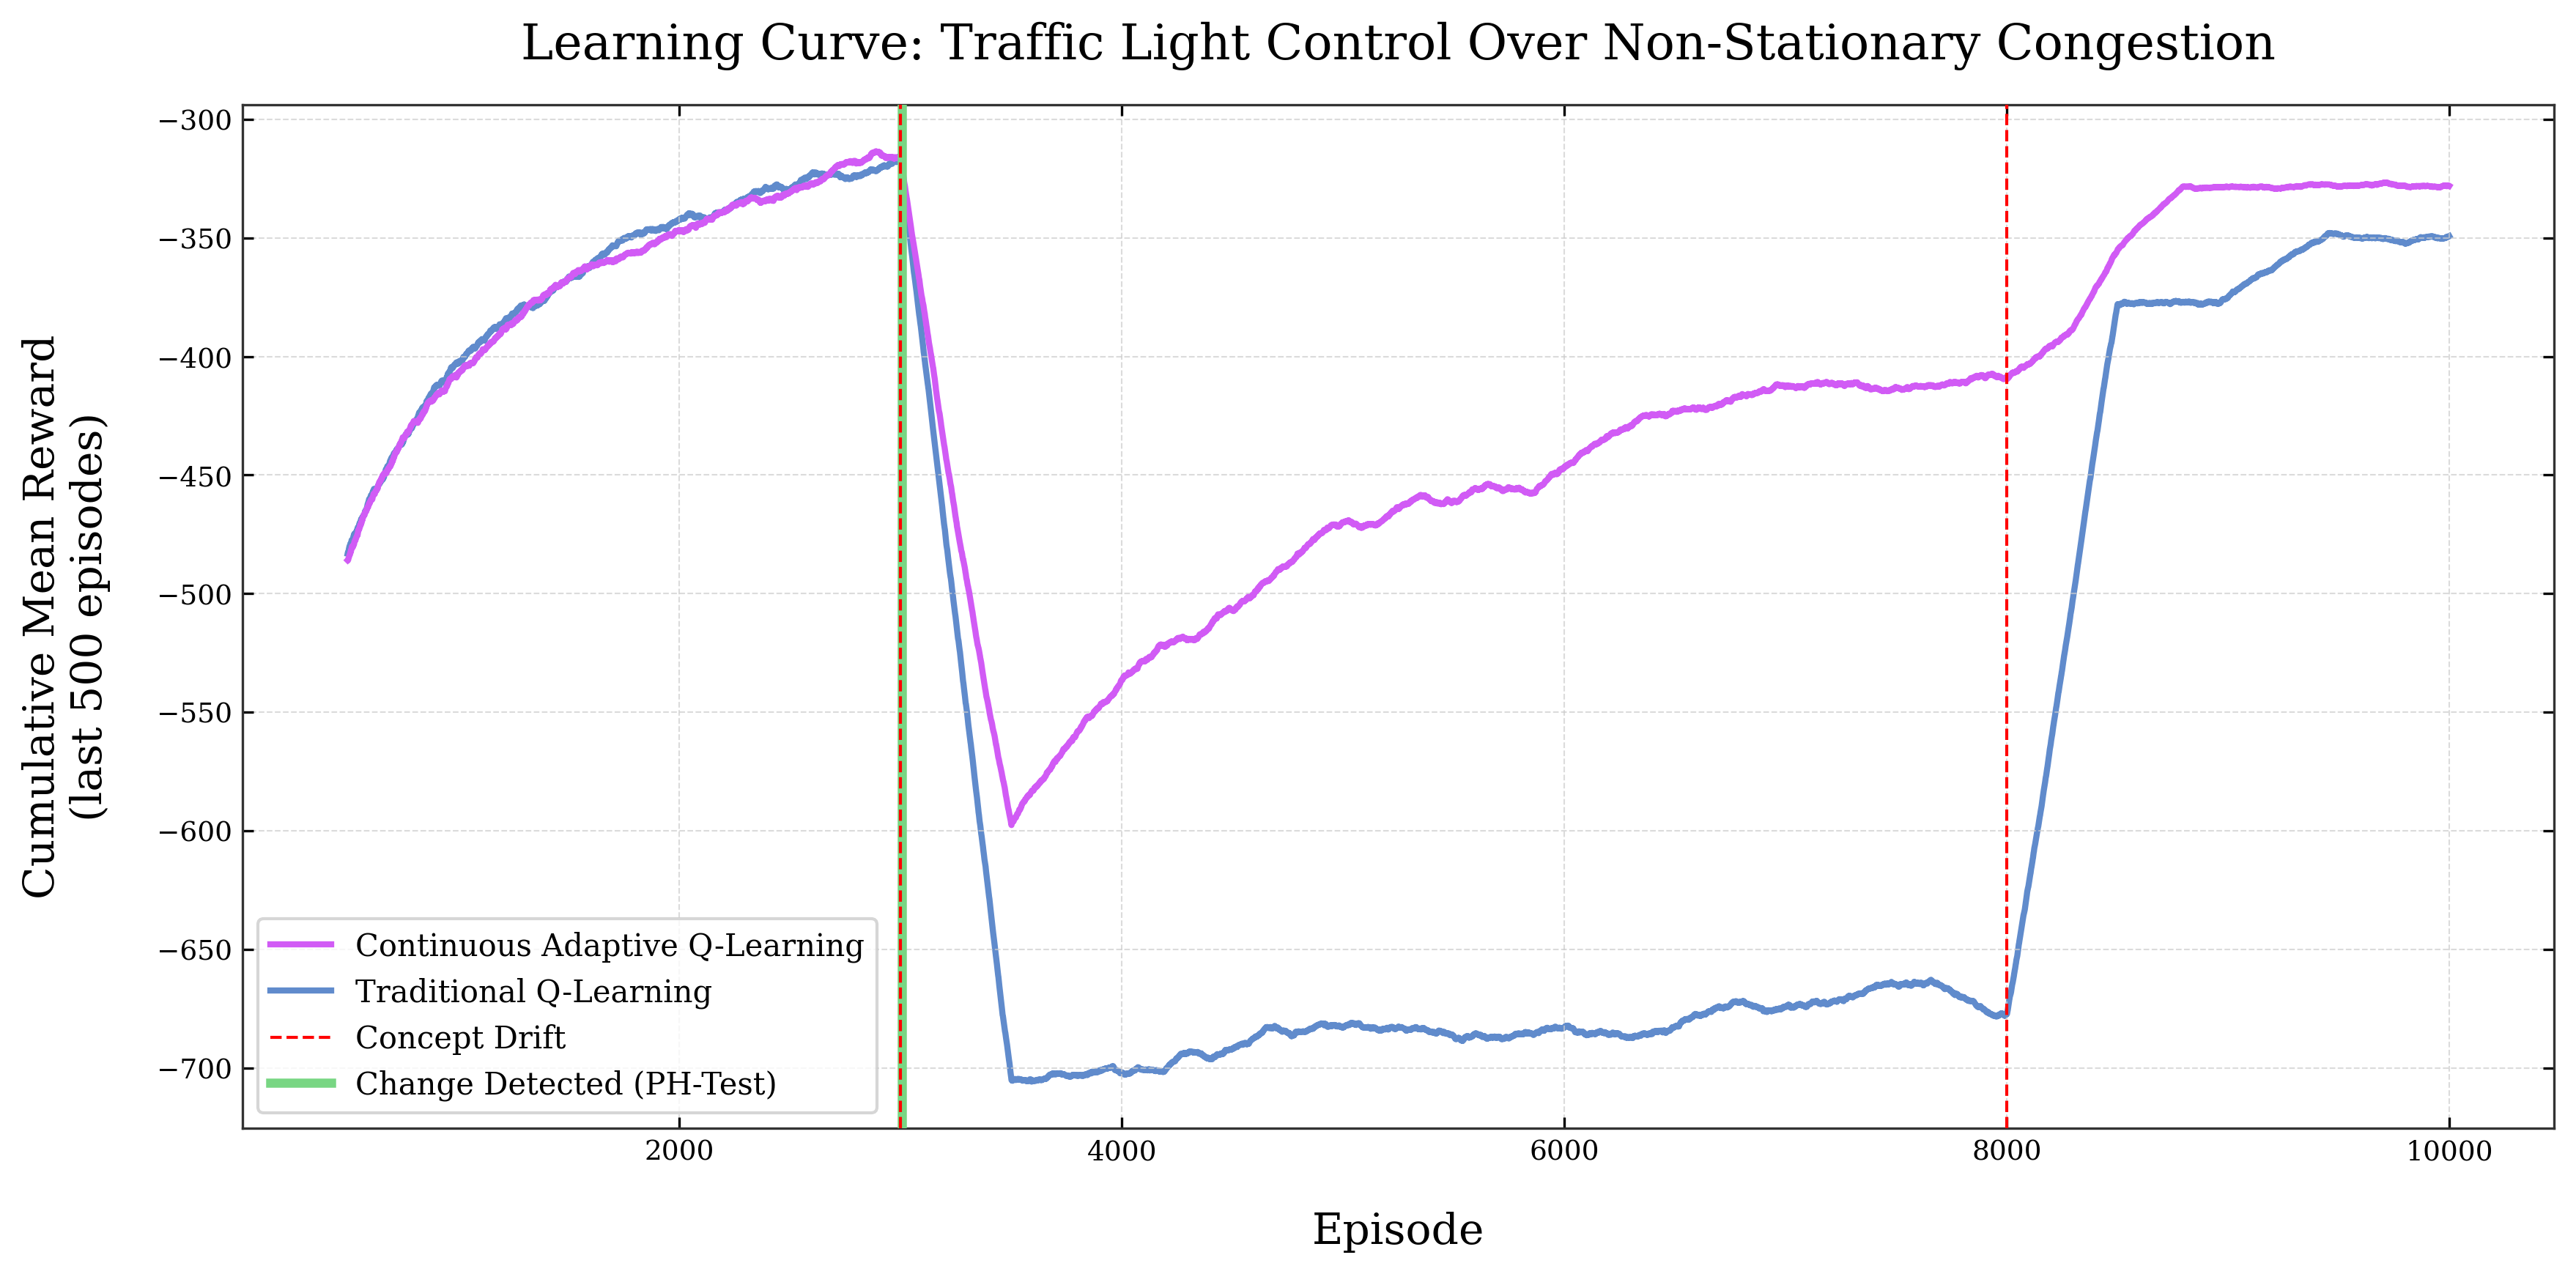
\includegraphics[width=\textwidth]{figures/traffic_learning_curve}
    \caption{Learning performance for traffic-signal control under non-stationary congestion. \adaptiverl rapidly recovers after the first drift thanks to extension of action set after PH-Test detection, while traditional Q-learning suffers prolonged performance drops.}
    \label{fig:traffic-learning-curve}
\end{figure*}

Initially, both agents improve steadily. After the first drift, \adaptiverl promptly increases exploration, exploits its new actions $(7,3)$ and $(3,7)$, and regains performance within a few hundred episodes. In contrast, the standard agent endures a deep, slow recovery. The built-in penalty for wasted green time ensures \adaptiverl does not “over-serve” when queues shrink, automatically balancing old and new phases without discarding any actions.

This traffic-signal case confirms that \adaptiverl can:
\begin{enumerate}
  \item Detect and react to non-stationary congestion via the PH-test, boosting exploration exactly when needed and the adaptive mechanisms that distinguish \adaptiverl.
  \item Seamlessly incorporate new signal phases---analogous to real-world reprogramming of traffic lights---without removing prior options.
  \item Leverage a dynamic reward (with penalization) to avoid excessive service when traffic is light, resulting in resource-efficient policies.
\end{enumerate}
In practice, modern traffic controllers can update phase timings in real time; endowing them with self-adaptive intelligence, as in \adaptiverl, allows continuous, automated adjustment to changing traffic patterns without manual retuning.


\endinput

